\documentclass[a4paper,12pt]{article}
\usepackage{amsmath}
\usepackage{amssymb}
\usepackage[polish]{babel}
\usepackage{polski}
\usepackage[utf8]{inputenc}
\usepackage{indentfirst}
\usepackage{geometry}
\usepackage{array}
\usepackage[pdftex]{color,graphicx}
\usepackage{subfigure}
\usepackage{afterpage}
\usepackage{setspace}
\usepackage{color}
\usepackage{wrapfig}
\usepackage{listings}
\usepackage{datetime}

\renewcommand{\onehalfspacing}{\setstretch{1.6}}

\geometry{tmargin=2.5cm,bmargin=2.5cm,lmargin=2.5cm,rmargin=2.5cm}
\setlength{\parindent}{1cm}
\setlength{\parskip}{0mm}

\newenvironment{lista}{
\begin{itemize}
  \setlength{\itemsep}{1pt}
  \setlength{\parskip}{0pt}
  \setlength{\parsep}{0pt}
}{\end{itemize}}

\newcommand{\linia}{\rule{\linewidth}{0.4mm}}

\definecolor{lbcolor}{rgb}{0.95,0.95,0.95}
\lstset{
    backgroundcolor=\color{lbcolor},
    tabsize=4,
  language=C++,
  captionpos=b,
  tabsize=3,
  frame=lines,
  numbers=left,
  numberstyle=\tiny,
  numbersep=5pt,
  breaklines=true,
  showstringspaces=false,
  basicstyle=\footnotesize,
  identifierstyle=\color{magenta},
  keywordstyle=\color[rgb]{0,0,1},
  commentstyle=\color{Darkgreen},
  stringstyle=\color{red}
  }

\begin{document}

\noindent
\begin{tabular}{|c|p{11cm}|c|} \hline 
Grupa 5 & Kamil Wanat, Dariusz Szczupak & \ddmmyyyydate\today \tabularnewline
\hline 
\end{tabular}


\section*{Zadanie 4 - Liczby Pierwsze OpenMP}

Zadanie laboratoryjne polegało na zaimplementowaniu programu sprawdzającego czy podane liczby są liczbami pierwszymi, czy złożonymi. Program w swoim działaniu wykorzystuje dyrektywy OpenMP w celu jego zrównoleglenia. Problem został rozwiązany przy pomocy Algorytmu sita Eratostenesa. Dzięki takiemu podejściu obliczenia są wykonywane jednokrotnie dla całego zbioru liczb. Przytoczony powyżej algorytm opiera swe działanie na eliminacji ze zbioru liczb które są podzielne przez kolejne liczby od 2 do pierwiastka kwadratowego z liczby testowanej. W naszym programie pierwiastek obliczany jest z liczby maksymalnej, dzięki czemu możemy przetestować wszystkie zdefiniowane w pliku liczby. To właśnie pętla odpowiedzialna za sprawdzanie kolejnych dzielników została zrównoreglona w programie. Poniżej znajduje się część zasadnicza programu ukazująca sposób ''odsiewania'' liczb złożonych.

\begin{lstlisting}
#pragma omp parallel for default(shared) private(i,j) num_threads(threadsCount) schedule(runtime)
    for (i=2;i<=sqr;i++) {
        for (j = 0; j <tab.size(); j++) {
                if((tab[j].value%i==0)&(tab[j].value!=i))
                    tab[j].prime=false;
        }
    }
\end{lstlisting}


Poniżej kodu znajduje się jego opis, który nie jest opisem w stylu "Tak, to nawet działa! Jest pętla i jest kolorowe. Szkoda, że się nie rusza. 

Poniżej kodu znajduje się jego opis, który nie jest opisem w stylu "Tak, to nawet działa! Jest pętla i jest kolorowe. Szkoda, że się nie rusza. 
Poniżej zamieszone są wykresy na dowód posiadania umiejętności obsługi pakietu biurowego Microsoft Office Excel lub LibreOffice Calc. Można tutaj również pochawlić się znajomością małego lecz potężnego programu gnuplot.

\begin{figure}[!hbp]
	\centering
  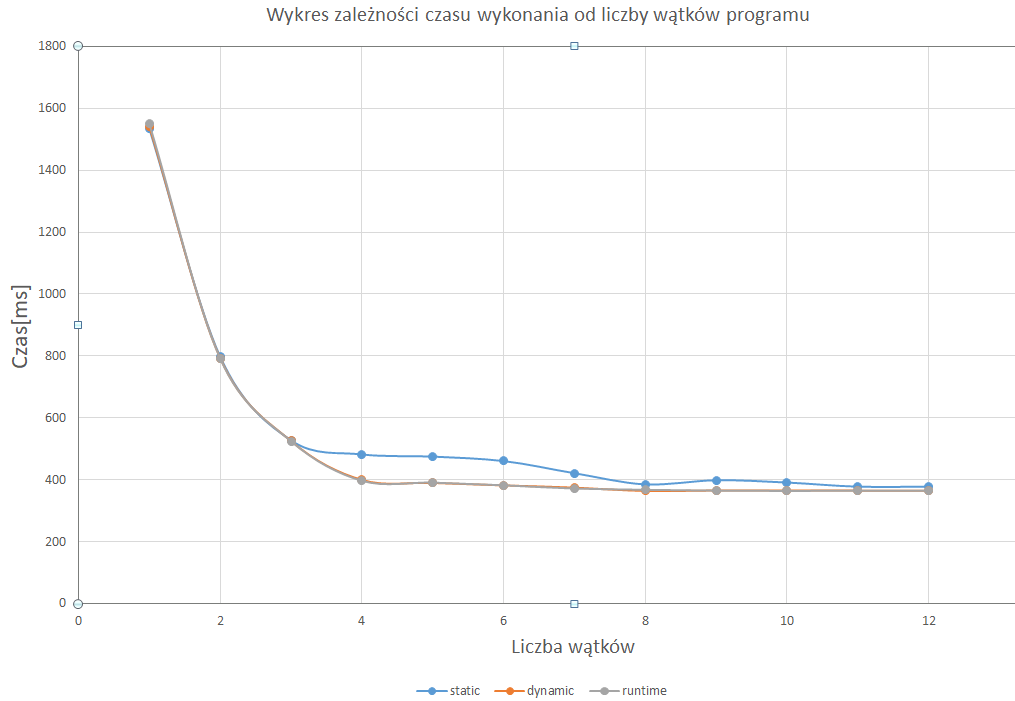
\includegraphics[width=0.7\textwidth]{wykres.pdf}
  \caption{Profesjonalna prosta czerwona kreska z kropkami}
\end{figure}

\begin{wrapfigure}{r}{0.5\textwidth}
  \vspace{-20pt}
  \begin{center}
  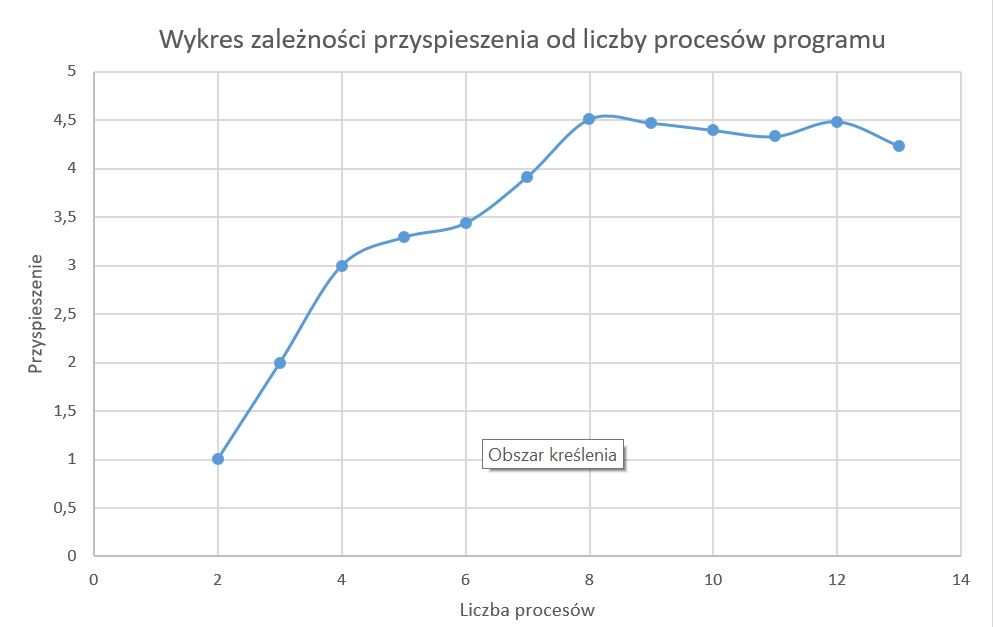
\includegraphics[width=0.45\textwidth]{wykres1.pdf}
  \end{center}
  \vspace{-20pt}
  \caption{Krzywa niebieska kreska}
  \vspace{-10pt}
\end{wrapfigure}


W celu ułatwienia pracy Prowadzącemu warto wykresy podpisać, aby Prowadzący omyłkowo nie przyjął, że dany wykres przedstawia średnią miesięczną temperaturę w Bangladeszu na przełomie lat 1975-1982, ponieważ taki wykres byłby nieodpowiedni, przez co sprawozdanie byłoby niezaliczone. Łatwo zauważyć, że każdy wykres w przestrzeni 2D posiada dwie osie i z grzeczności należy je opisać. Osie posiadają jednostki, które też warto przytoczyć.

Czasem w sprawozdaniu warto przytoczyć kilka zalet danego rozwiązania i wypisać je jako lista:
\begin{lista}
 \item Pierwszą zaletą jest to, że jest.
 \item Druga zaleta jest również obecna.
 \item Trzecia zaleta jest już troche naciągana.
 \item Czwarta zaleta jest wadą, czyli zaletą ujemną.
\end{lista}

Jeśli zaszłaby konieczność zestawienia danych wartości w tabeli to również jest taka możliwość.

\begin{table}[!hbp]
\centering
\begin{tabular}{|p{5cm}|c|}
\hline 
Zalety & Wady \tabularnewline
\hline 
 Ładne, kolorowe & Brak\tabularnewline
 Szybkie, działające & Brak\tabularnewline
\hline
\end{tabular}
\caption{Podpis bardzo wartoścowej tabeli z danymi}
\end{table}


W sprawozdaniu muszą znaleźć się wnioski. Wnioski stanowią przesłankę, o tym iż osoba je pisząca, która ubiega się o tytuł magistra inżyniera, wie co robi. Osoba taka często jest w stanie określić czemu miało służyć dane ćwiczenie, a także ocenić w jakim stopniu udało się rozwiązać dane zagadnienie i gdzie napotkano problemy.

\end{document}
